\documentclass[12pt]{report}

\usepackage{amsmath} % for equations
\usepackage{graphicx} % for adding images
\usepackage[margin=1.0in]{geometry} % make margins smaller
\usepackage{listings} % for code blocks
\usepackage{hyperref} % for links
\usepackage{setspace} % for line spacing
\usepackage{indentfirst}
\usepackage{titling} % for multiple title pages
\usepackage{placeins}   % for \FloatBarrier, helps divide sections

\linespread{1.5}
%\doublespacing

\pretitle{\begin{center}\huge}
\posttitle{\par\end{center}\vspace{\baselineskip}}
\preauthor{\normalfont\normalsize\begin{center}\begin{tabular}[t]{c}}
\postauthor{\end{tabular}\end{center}\vspace{\baselineskip}}

\title{CSCE 465 Cryptography in Action}
\date{}

\begin{document}
\maketitle

\newpage
\author{Nathan Brockway\\Dominick Fabian\\Blake Nelson}
\date{Submitted: December 8, 2018}
\maketitle

\tableofcontents
\newpage

\begin{abstract}
    Since as early as the ancient Roman days, secret messages have been sent from a command post to the front during wartime. With the constant risk of messengers
    being captured and their messages intercepted, a method of ensuring that only the authorized parties were able to read messages has been necessary. Such is the
    beginning of cryptography and the battle to devise new ways to break cryptographic systems. This project seeks to demonstrate the strengths and weaknesses in
    current popular cryptographic systems such as RSA, El Gamal, and DES. To do this, a client and a server are connected over the TCP/IP stack and exchange
    information. The client will send an encrypted message to the server, and the server will decrypt this and respond back with its own encrypted message. The
    client will then be able to decrypt and read this reply. Meanwhile, a malicious user will capture the encrypted communications en route and attempt to break the
    cryptographic system. To do this, a brute force and a more intelligent method will be used to recover the plaintext from the ciphertext. In this report, we
    analyze and discuss the performance of each of these attack vectors on a number of cryptosystems. Unsurprisingly, the brute force attacks on encryption are not
    nearly as effective as more sophisticated attacks that extort some of the weaker mathematical properties of the cryptosystems. These results are summarized in
    graphs and explained in depth in this report.
\end{abstract}


\chapter{Final Report}
% for the progress report and the final report
\section{Introduction}
Mathematicians and computer scientists have spent years developing new algorithms that allow for the safe transfer of information from one party to another.
These algorithms have come down to two main approaches: symmetric key encryption, where both parties share a single key used to encrypt and decrypt a message,
and public key encryption, where both parties use a common key for encryption, but also have their own, private keys used in decryption. In our schooling, we
have learned algorithms using both approaches, either during this course or in MATH 470 - Communications and Cryptography. In this project, we will implement a few
of these algorithms using Python and TCP sockets, and evaluate their effectiveness. We will first demonstrate the efficiency of the algorithm: how long it
takes to get from plaintext to plaintext end to end compared to the length of the key. Next, we will use implement approaches learned both in this course and
in MATH 470 to decipher the key. These approaches utilize either a known plain text/cipher text combination to randomly guess the key, or take advantage of the
public key to perform mathematical operations and decipher the key in a more structured fashion. By timing both the message transfer and the ability to crack the
decryption, we will put together a comprehensive study on the effectiveness of the algorithms individually and form a comparison between symmetric key encryption
and public key encryption. Finally, we evaluate the efficiency and effectiveness of the Digital Signature Algorithm (DSA).

% for the progress report and the final report
\section{Background and Literature Review}
Both cryptosystems have long histories. Public key cryptography was first conceptualized in the early 1970s by British cryptographers working for the UK Government
Communications Headquarters. Clifford Cocks developed what is currently known as the RSA algorithm in 1973 \cite{class}. This method was shared with the US, along
with a key exchange method, and was used in secret for many years. Later, in 1985, three scientists at MIT - Ron Rivest, Adi Shamir, and Leonard Adleman - published
a generalized version of Cocks' algorithm, coining the name "RSA" after their initials. While the works of Cocks and others was the true first discovery of this
cryptography method, the classified nature of the work kept them from getting their proper credit. At the same time as RSA, another public key cryptography method
was published by Taher Elgamal \cite{elgamal}, using discrete logs instead of the prime factorization of RSA to remain secure.

Meanwhile, symmetric key encryption was based on the One Time Pad encryption scheme, and the similarities are apparent, as many stream and block ciphers (two
approaches to symmetric encryption) are based on each bit, or block, being used in an exclusive-OR operation. One Time Pad and block ciphers can be traced back
to as early as 1949 when it was first proven to be secure. The Data Encryption Standard (DES) is a well known symmetric key algorithm, dating back to 1975 when
it was first published, but there are more recent algorithms such as AES, published in 1998. DES is based on the Feistel cipher, a project done by Horst Feistel
during his time at IBM \cite{feistel}. Feistel's method uses a fixed key size on message blocks of the same size, repeating the function until the end of the
message. DES employs the same scheme, making it a common block cipher. DES and many other block ciphers can have different modes of encryption \cite{modes}. These
modes vary how the plain text and cipher text blocks interact and their dependencies. Making blocks dependent on the previous output allow for propagation in
encryption, so that equivalent plain text blocks do not always produce the same cipher text blocks for each message. While this project will not focus on the many
different modes of operation, it will public and secret key cryptography methods into a comprehensive review of effectiveness and efficiency.

In addition to the need to keep messages secret while they are en route, there is a need to verify authenticity of a message. Verifying that a message was indeed
sent from the person that they claim to be is arguably as important as sending the message itself. Very similar to one adding one's written signature to the bottom
of a document to signify his or her agreement with the document, digital signatures work much the same way. This digital signature took the form of the Digital
Signature Algorithm (DSA) in 1991 with support from the U.S. Government.\cite{mit}\cite{dsa}

\section{Method and Approach}
% TODO: specify how the code is written and how the attacks work
The source code for the project is organized into Python classes for Encryption, Decryption, Signature, and Attack. Each of the classes takes in as a parameter the
type of algorithm to use and the string of characters to perform the action on. To complete a simulated transaction, the client will use the Encryption module to
encrypt and send a message to the server. The server will use the Decryption module to read the message and the Encryption module to formulate and send a response.
Then the client uses the Decryption module to read the response. All the while, the attacker is using the Attack module to try to read the two ciphertexts after
capturing the TCP packets. This is the basic format of the attacks and benchmarks are taken to see how long each encryption, decryption, and attack takes. The source
code for our approach can be found in Appendix A.

\subsection{Attacking RSA}
The strength of RSA comes from the idea that it is difficult to factor a large product of two primes. Since this has been deemed computationally infeasible, the
security of the cryptosystem is based completely on this idea. This means that if $n$ can be factored, then RSA-encrypted communications are no longer secure.
Before discussing the methods attempted to factor a product of two large primes, let us first understand why RSA relies on the secrecy of these prime factors.

As RSA is a public key cryptosystem, each user in the system has both a public and a private key. The public key is denoted $(e,n)$ and the private key is denoted
$(d,n)$, where $n$ is the product of two large primes and $e,d$ are the encryption and decryption exponents, respectively. $n$ is made by multiplying two large
primes, $p$ and $q$. Then the Euler totient of $n$, $\phi(n)$, is calculated as $\phi(n) = (p-1)(q-1)$. This is used to calculate $e$ and $d$ such that
$ed \equiv 1$ (mod $\phi(n)$). Since $e$ and $n$ are made public to the whole world, finding $\phi(n)$ would allow anybody to calculate the decryption exponent and
thereby both decrypt all communications encrypted with the corresponding public key and impersonate the holder of the private key. In order to calculate $\phi(n)$,
the prime factors $p$ and $q$ need to be found. Thus, the idea that finding such factors of $n$ is difficult remains as the basis of the RSA cryptosystem.

The number of primes less than a given number $x$ can be approximated as $\frac{x}{ln(x)}$. If a 2048-bit RSA key were to be used, this number would have about 617
digits in base 10. This means that there are a \textbf{huge} number of potential prime numbers that could be factors of $x$ and it would take a \textbf{very} long
time to try them all, even for a powerful computer.

For this project, two methods of factoring $n$ were explored: brute-force guessing and Pollard's $p-1$ method.\cite{pollard} Our brute force implementation took the
ultimate naive approach and simply tries every single odd number less than $n$ until it found the smaller of the factors. Once it found one of the factors of $n$,
it was trivial to find the other factor and $\phi(n)$ was easily calculated. By taking an inverse mod of $\phi(n)$ using the known encryption exponent, $e$, any
ciphertext created with $d$ could then be decrypted.

Pollard's $p-1$ method takes a much more intelligent approach. Instead of trying to guess the small prime in the composite $n$, we started with $a=2$ and set a bound
$B$ to be around 100 or so. Then we calculated $b=2^{B!}$ (mod $n$). If $gcd(b-1,n)$ was not 1 or $n$, then we have found a non-trivial factor of $n$. If we did not
get a non-trivial factor of $n$, we simply increased the size of our bound $B$ and tried again. For larger key sizes, a larger $B$ must be used. Varying $a$ is also a
valid approach to factorize $n$. The method works because of Fermat's Little Theorem, a very important theorem in number theory. Since $(p-1)|B!$, this implies that
$B!$ is an integer multiple of $(p-1)$. From this, we see that $b \equiv 2^{B!}$ (mod $p$) $\equiv 2^{k(p-1)}$ (mod $p$) $\equiv$ 1 (mod $p$) and it is easy to get
a prime factor from $p-1$ by adding 1. The bottleneck of the Pollard method is how quickly you can calculate $2^{B!}$ (mod $p$) since the factorial makes the amount
of computation grow at beyond exponential rates!

For a comparison of the two attacks on RSA, see section \ref{results}.

\subsection{Attacking El Gamal}
Just as RSA relies on the computational infeasibility of factoring products of large primes, El Gamal relies on what is known as the Discrete Logarithm Problem. The
premise of this problem is that given the congruence $a^{x} \equiv b$ (mod $n$) and that $n$ is prime, for some known $a^{x}$, $b$, and $n$ there is no efficient
way to find $x$. Also, a must be a primitive root of n which ensures no message collisions \cite{root}. However, there are still some methods of recovering a
plaintext from an El Gamal ciphertext of various effectiveness. For this project, we experiment with brute-force, the Pohlig-Hellman method, and the Shank's method.

The brute force attack on El Gamal is even more naive then the brute force of RSA since the private key $x$ can be any number from $2$ to $p-2$ inclusively.
Therefore, the larger prime $n$ is in the public key the more possibilities for $x$ and the more computational time the brute force attack takes.

The Shank's and Pohlig-Hellman attacks on El Gamal both utilize a rainbow table type of attack. This style of attack focuses on finding a single variable answer
by expressing that variable, in this case $x$ the private key, as a two or more variable equation. Then generating all possibilities of the new equation and using
the two variables to find the single variable. Shank's method for attacking El Gamal first picks $N > \sqrt{n}$ then generates to lists: list j where
$entry \equiv a^{j}$ (mod $n$) where $j \in (1,N)$ and list k where $entry \equiv ba^{-Nk}$ (mod $n$) where $k \in (1,N)$. Due to the choice of $N$ and $a$ is a
primitive root of $n$, it is certain that a match exists in the two lists. Then using the indices of the match, the private key can be found by $x = j + N*k$. This
approach is also know as a "Baby-Step Giant-Step" attack since the j-list takes small steps and the k-list takes $N$ sized steps.

The Pohlig-Hellman approach uses Shank's "Baby-Step Giant-Step" idea but instead divides the problem into finding the answers to $x$ (mod $p$) where
$p \in factors(n-1)$. This information is useful because of the Chinese Remainder Theorem, CRT. This theorem states that given $k \equiv a$ (mod $x$) and
$k \equiv b$ (mod $y$) $\exists c$ where $k \equiv c$ (mod $xy$). Therefore, using CRT to combine the answers to $x$ (mod $p$) where $p \in factors(n-1)$, one can
calculate $x$ (mod $n-1$) and since the private key $1 < x < n-1$ then $x$ (mod $n$) is the solution. However, similar to Pollard's $p-1$ attack on RSA this attack
relies on $n-1$ having small prime factors to be efficient.

\subsection{Attacking DSA}
The Digital Signature Algorithm relies on the same premise of El Gamal where solving the Discrete Log Problem is hard. However, the keys of El Gamal and DSA are
very different because for $a^{x} \equiv b$ (mod $n$) El Gamal requires a to be a primitive root of n but DSA requires a not to be a primitive root but
$a \equiv g^{(n-1)/q}$ (mod $n$) where q is the largest prime factor of $n-1$. This requirement ensures that attacks on El Gamal cannot be used on DSA and the
signature algorithm of DSA produces signatures with no collisions. Attacks on DSA are widely undeveloped due to a lack of mathematical discovery around the Discrete
Log Problem. One of the best current rigorous approaches utilizes Lagrange Lattice Reduction to produce a solution in polynomial time \cite{lattice}. However, a
more efficient approach is a birthday attack where one computes random permutations of private key $x$ and random integer $k$, used in the signature algorithm of
DSA, to increase the probability of generating an intercepted signature. This approach, however, is probabilistic but does run in $O(\sqrt{n})$ time.

\subsection{Attacking DES}
DES is a symmetric key algorithm designed in 1975 in conjunction with the U.S. Government. While no longer considered to be a safe algorithm for sensitive
information, its popularity in past years makes it worthwhile to attack and benchmark. DES takes in a 64-bit key and uses this key to create 16 sub-keys to be used
in each round of the DES encryption. The algorithm was designed to be easy to implement in hardware and difficult to implement in software, so this proved a bit of
a challenge to design in our Python scripts and is going to be significantly slower running in software than it would be using actual DES hardware.

For this project, we experiment with a brute force attack on DES. To do this, we first need a known plaintext/ciphertext pair. Once we have this, we
generate a random set of keys, encrypt the plaintext, and check to see if the result is the ciphertext. If we get the ciphertext from the pair as a result, then we
have found the key needed to generate the DES key sets. If the result does not match the known cipher text, the key is linearly incremented, a new set of keys is
generated, and the known plaintext is encrypted again. This approach was continuously repeated until the resulting cipher was equivalent to the known cipher. This
brute force approach was repeated for keys of different digit sizes, similar to the other approaches in this project. The results can be seen in section \ref{results}.

\subsection{Attacking One-Time Pad}
The One-Time Pad is the only cryptosystem tested in this project that is perfectly secure. The reasoning behind this claim is that it is impossible to do any better
than a brute force attack on the algorithm. This is because the key-space is the same size as the message-space. Each bit of the message is XOR'ed with a bit of the
key, so there is no real math involved that could be exploited. The only way to recover the plaintext from the ciphertext is to know the key. The only way to know
the key is to guess every single key of the same length as the message until you get it (assuming that the key is only used the one time). The approach to this
algorithm is the same as the DES approach above. A known plain text and cipher text is obtained, encrypted with a key of a certain digit length. The attacker then
obtains this pair, and linearly searches for a key that encrypts the known plain text correctly. Because the encryption key is random and dependent on the length of
the message, several benchmark runs had to be conducted to obtain comprehensive results for a reasonable range of key lengths. These results were merged together, and
can be seen in section \ref{results}.

\section{Results}
\label{results}

All of the graphs showing the results of the project testing can be found in Figures \ref{fig:allattack}--\ref{fig:TransferBenchmarks}. A comprehensive illustration of
all algorithms and their attacks is shown in figure \ref{fig:allattack}. According to the graph, the encryption system most resilient to attacks is El Gamal, since the
time to guess the key becomes exponential the fastest, and is the quickest to reach a point of computational infeasibility in regards to this project. El Gamal also
comes in second in this graph, this time using Shank's algorithm of deriving the key. This approach is more complex, but still reaches computational infeasibility
quickly. Following this line on the graph is the brute force for RSA encryption. Since this attack only has to search values up to the square root of $n$, this result
is expected. The next most difficult attack per the graph is the Pohlig-Helman algorithm on El Gamal encryption. This attack improves on Shank's algorithm, but improves
it with the use of the Chinese Remainder Theorem, so it makes sense that the graph would show it to be more efficient. The last attack on the graph is the $p-1$ attack.
Since this attack has shorter computations and a more mathematical approach to searching for a factor than linearly scanning, it can be expected to be the most efficient
algorithm in this project.

Figures \ref{fig:rsa1}--\ref{fig:el-gamal1} show the individual results of brute force attacks against all algorithms implemented in this project, in more detail than the
comprehensive figure described above. The symmetric key encryption schemes became exponential very quickly, and becoming infeasible at 12 digits for DES (fig.
\ref{fig:DESBruteForce}) and 7 digits for One Time Pad (fig. \ref{fig:OTPBruteForce}). This is a result of the randomness of the key, or the message length in the case of
One Time Pad. Following these algorithms, the brute force attack on El Gamal encryption was the next closest, becoming out of scope when a prime number of 10 digits was
used, according to figure \ref{fig:el-gamal1} Finally, the brute force attack on RSA was the most efficient, becoming infeasible with a prime number of 22 digits according
to figure \ref{fig:rsa1}.

While brute force attacks are the easiest to implement, there are others that are proven to be more efficient. Figure \ref{fig:rsa2} shows one such attack on RSA encryption.
There are some large spikes in the data, but in general the data shows that RSA encryption can be broken in under a few minutes, despite using a prime of 30 digits long.

Algorithms against the discrete logs that El Gamal encryption is based on were recorded as well. Figures \ref{fig:el-gamal2} and \ref{fig:el-gamal3} show two algorithms
that derive these keys much faster than a brute force attack. According to figure \ref{fig:el-gamal2}, Shanks's algorithm was able to derive keys using primes up to 16
digits long before becoming unfeasible. The Pohlig-Helman attack was even more efficient, deriving keys based on primes of 23 digits in length before becoming unfeasible,
as illustrated in figure \ref{fig:el-gamal3}.

The last benchmark data recorded was the time it would take to encrypt and decrypt data using each encryption scheme, to test efficiency. Generally, symmetric key encryption
is faster than its public key counter part due to the complexity of the algorithms, and this statement is supported by the graph in figure \ref{fig:TransferBenchmarks}. Both
One Time Pad and DES stay close to the bottom, requiring little computation to perform their duties. Meanwhile, RSA can be seen slowly rising in time as the key reaches 20
digits in length. And while the timing doesn't follow a clear trend on it's own, El Gamal encryption is noticeably higher in time than the rest of the group, reaching times
that are magnitudes higher than its counterparts for equivalent key sizes.
\\
\\
\\

\begin{figure}[hp!] % [hp!] means ''here''
    \begin{center}
        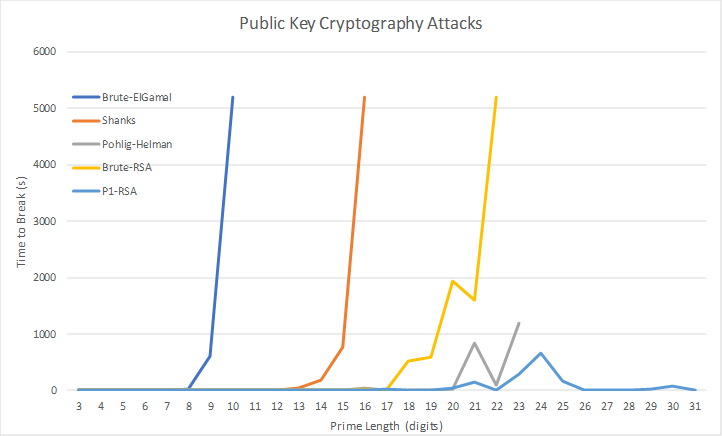
\includegraphics[width=0.85\linewidth]{AllAttack.PNG}
        \caption{Comparison of All Attacks Tested}
        \label{fig:allattack}
    \end{center}
\end{figure}

\begin{figure}[hp!] % [hp!] means ''here''
    \begin{center}
        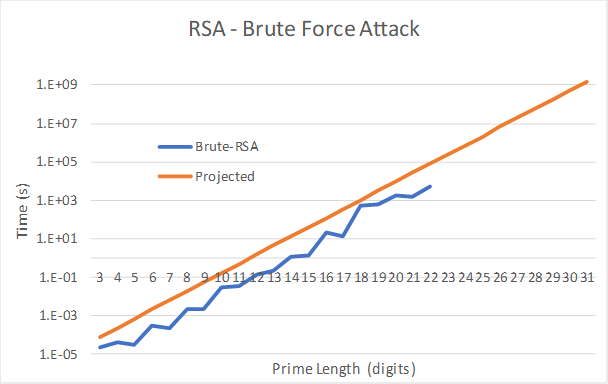
\includegraphics[width=0.85\linewidth]{RSABrute.PNG}
        \caption{Brute Force Attack on RSA}
        \label{fig:rsa1}
    \end{center}
\end{figure}

\begin{figure}[hp!] % [hp!] means ''here''
    \begin{center}
        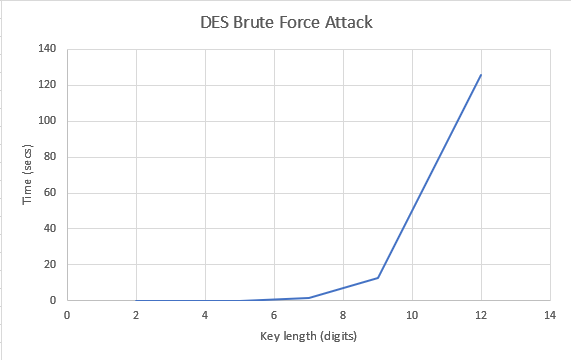
\includegraphics[width=0.85\linewidth]{DESBruteForce.png}
        \caption{Brute Force Attack on DES}
        \label{fig:DESBruteForce}
    \end{center}
\end{figure}

\begin{figure}[hp!] % [hp!] means ''here''
    \begin{center}
        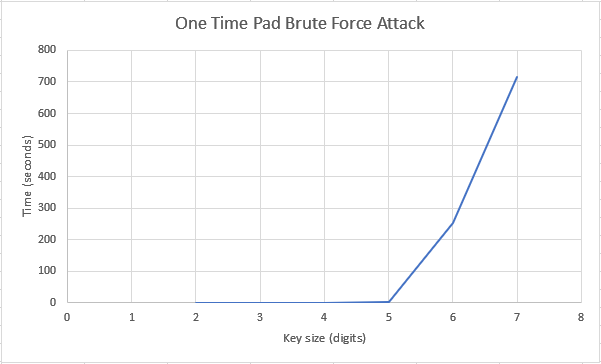
\includegraphics[width=0.85\linewidth]{OTPBruteForce.png}
        \caption{Brute Force Attack on One Time Pad}
        \label{fig:OTPBruteForce}
    \end{center}
\end{figure}

\begin{figure}[hp!] % [hp!] means ''here''
    \begin{center}
        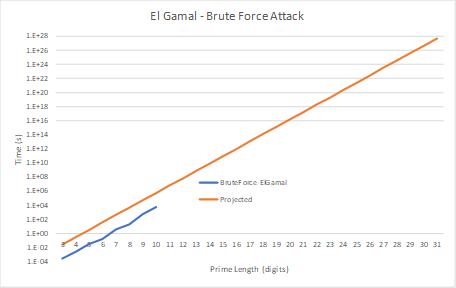
\includegraphics[width=0.85\linewidth]{ElGamalBrute.PNG}
        \caption{Brute Force Attack on El Gamal}
        \label{fig:el-gamal1}
    \end{center}
\end{figure}

\begin{figure}[hp!] % [hp!] means ''here''
    \begin{center}
        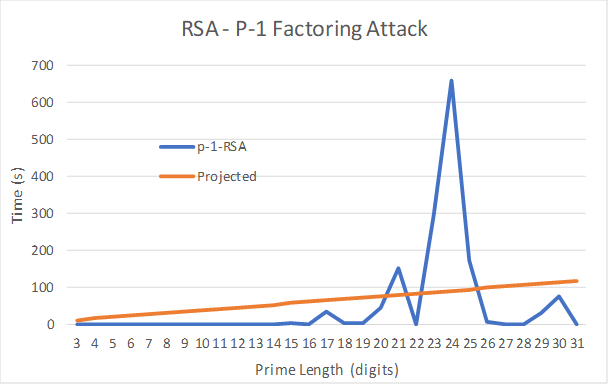
\includegraphics[width=0.85\linewidth]{RSAp-1.PNG}
        \caption{$p-1$ Attack on RSA}
        \label{fig:rsa2}
    \end{center}
\end{figure}

\begin{figure}[hp!] % [hp!] means ''here''
    \begin{center}
        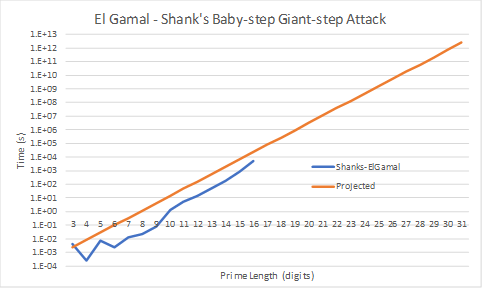
\includegraphics[width=0.85\linewidth]{ElGamalShanks.PNG}
        \caption{Shank's ``Baby-Step Giant-Step'' Attack on RSA}
        \label{fig:el-gamal2}
    \end{center}
\end{figure}

\begin{figure}[hp!] % [hp!] means ''here''
    \begin{center}
        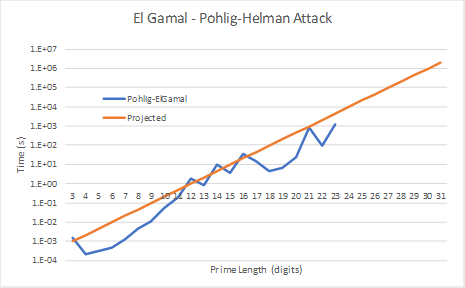
\includegraphics[width=0.85\linewidth]{ElGamalPohlig.PNG}
        \caption{Pohlig-Hellman Attack on El-Gamal}
        \label{fig:el-gamal3}
    \end{center}
\end{figure}

\begin{figure}[hp!] % [hp!] means ''here''
    \begin{center}
        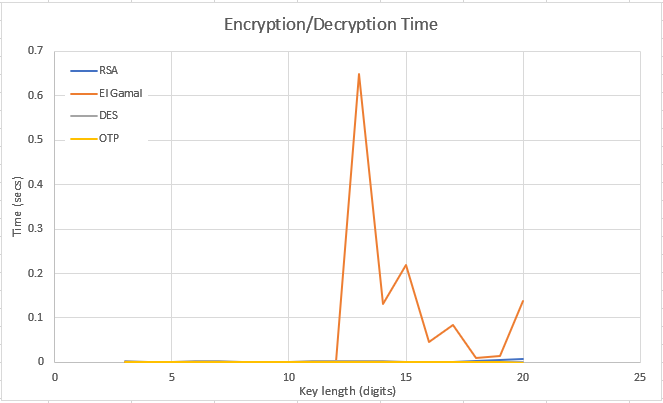
\includegraphics[width=0.85\linewidth]{TransferBenchmarks.png}
        \caption{Time to encrypt and decrpyt a message with each algorithm}
        \label{fig:TransferBenchmarks}
    \end{center}
\end{figure}
\FloatBarrier
\section{Discussion and Recommendations}
As shown in the Results section of this report, the brute force attacks were significantly slower than the more informed attacks on the cryptosystems. However,
despite the relative ineffectiveness of the brute force attacks, they were still relatively effective against RSA. Figure \ref{fig:allattack} best shows this data.
Here, we see that El Gamal is much more resistant to brute force attacks than RSA is. Additionally, the $p-1$ factorization attack is by far more successful than
the Shanks' and Pohlig-Hellman attacks on El Gamal. This seems to point to the idea that El Gamal is overall more resistant to attack than RSA is, so this research
team recommends the use of El Gamal over RSA for more sensitive information sent over insecure channels.

For the testing of DES, there was the question of how to simulate the testing of various key sizes for the algorithm, since the standard requires 64-bit keys.
However, to simulate smaller keys for our attacks, we created algorithms to generate keys of varying strengths. Keys with many leading zeroes are considered weaker
keys and more random-valued keys are considered stronger keys.

\section{Conclusion}
Brute force attacks are significantly slower than more informed attacks, such as Pollard's $p-1$ attack on RSA and Shanks' ``Baby-Step Giant-Step'' attack on El
Gamal. Additionally, all attacks on every cryptosystem becomes significantly more difficult when the size of the encryption key increases. In most cases, the
increase in computational complexity increases at an exponential rate. Overall, the One-Time Pad was the most secure cryptosystem under test, followed by El Gamal,
RSA, and DES.

In terms of the efficiency of sending messages, secret key (symmetric key) encryption was faster than public key (asymmetric key) encryption. This is likely due to
the fact that the iterative exponentiation and modulus division takes much more time than simple XORs and reordering of bit sequences. This explains why most
internet connections are initiated with public key communications to perform the key exchange, and then use symmetric key encryption from then on out.

% an example bibliography
\newpage

\begin{thebibliography}{9}

    \bibitem{class}
    Tom Espiner. 2010. GCHQ pioneers on birth of public key crypto. (October 2010). Retrieved November 27, from \\
    \texttt{https://www.zdnet.com/article/gchq-pioneers-on-birth-of-public-key-crypto/}

    \bibitem{first-ten}
    The First Ten Years of Public-Key Cryptography\\
    \texttt{https://cr.yp.to/bib/1988/diffie.pdf}

    \bibitem{elgamal}
    A Public Key Cryptosystem and a Signature Scheme Based on Discrete Logarithms.\\
    \texttt{https://ieeexplore.ieee.org/document/1057074/}

    \bibitem{rsa}
    A Method for Obtaining Digital Signatures and Public-Key Cryptosystems\\
    \texttt{https://people.csail.mit.edu/rivest/Rsapaper.pdf}

    \bibitem{feistel}
    Horst Feistel. 1973. Cryptography and Computer Privacy. Scientific American 228, 5 (May 1973), 15-
    23. DOI: \\
    \texttt{http://dx.doi.org/10.1038/scientificamerican0573-15}

    \bibitem{modes}
    DES Modes of Encryption. \\
    \texttt{https://csrc.nist.gov/csrc/media/publications/fips/81/archive/1980-12-02/documents/fips81.pdf}

    \bibitem{philzimmerman}
    Why I Wrote PGP.\\
    \texttt{https://www.philzimmermann.com/EN/essays/WhyIWrotePGP.html}

    \bibitem{stanford}
    The Diffie Hellman Problem.\\
    \texttt{https://crypto.stanford.edu/\~{}dabo/pubs/papers/DDH.pdf}

    \bibitem{mit}
    A Method for Obtaining Digital Signatures and Public Key Cryptosystems.\\
    \texttt{https://people.csail.mit.edu/rivest/Rsapaper.pdf}

    \bibitem{pollard}
    Notes on Pollard's $p-1$ Attack on RSA\\
    \texttt{https://www.math.columbia.edu/\~{}goldfeld/PollardAttack.pdf}

    \bibitem{dsa}
    Digital Signature Standard (DSS)\\
    \texttt{https://web.archive.org/web/20131226115544/http://csrc.nist.gov/\\publications/fips/fips1861.pdf}

    \bibitem{sieve}
    Function Field Sieve Method for Discrete Logarithms over Finite Fields.\\
    \texttt{https://www.sciencedirect.com/science/article/pii/S0890540198927614?via\%3Dihub}

    \bibitem{root}
    Primitive Root Testing.\\
    \texttt{http://www.apfloat.org/prim.html}

    \bibitem{lattice}
    Lattice Attacks on DSA. \\
    \texttt{https://eprint.iacr.org/2016/058.pdf}

\end{thebibliography}

\newpage
\section{Appendix A: Source Code}
All of the source code for this project can be found at:

\href{https://github.com/NelsonBlakeN/CryptoInAction}{https://github.com/NelsonBlakeN/CryptoInAction}.

\newpage
\section{Appendix B: Presentation Slides}

\end{document}
